%%%%%%%%%%%%%%%%%%%%%%%%%%%%%%%%%%%%%%%%%%%%%%%%%%%%%%%%%%%%%%%%%%
%%%%%%%% ICML 2016 EXAMPLE LATEX SUBMISSION FILE %%%%%%%%%%%%%%%%%
%%%%%%%%%%%%%%%%%%%%%%%%%%%%%%%%%%%%%%%%%%%%%%%%%%%%%%%%%%%%%%%%%%

% Use the following line _only_ if you're still using LaTeX 2.09.
%\documentstyle[icml2016,epsf,natbib]{article}
% If you rely on Latex2e packages, like most moden people use this:
\documentclass{article}

% use Times
\usepackage{times}
% For figures
\usepackage{graphicx} % more modern
%\usepackage{epsfig} % less modern
\usepackage{subfigure}

% For citations
\usepackage{natbib}

% For algorithms
\usepackage{algorithm}
\usepackage{algorithmic}

% Maths
\usepackage{amsmath}
\usepackage{amssymb}

% As of 2011, we use the hyperref package to produce hyperlinks in the
% resulting PDF.  If this breaks your system, please commend out the
% following usepackage line and replace \usepackage{icml2016} with
% \usepackage[nohyperref]{icml2016} above.
\usepackage{hyperref}

% Packages hyperref and algorithmic misbehave sometimes.  We can fix
% this with the following command.
\newcommand{\theHalgorithm}{\arabic{algorithm}}

% Employ the following version of the ``usepackage'' statement for
% submitting the draft version of the paper for review.  This will set
% the note in the first column to ``Under review.  Do not distribute.''
\usepackage{icml2016}

% Employ this version of the ``usepackage'' statement after the paper has
% been accepted, when creating the final version.  This will set the
% note in the first column to ``Proceedings of the...''
%\usepackage[accepted]{icml2016}


% The \icmltitle you define below is probably too long as a header.
% Therefore, a short form for the running title is supplied here:
\icmltitlerunning{Deep Manifold Learning on Music Audio for Navigating Large Sound Libraries}

\begin{document}

\twocolumn[
\icmltitle{Deep Manifold Learning on Music Audio \\
           for Navigating Large Sound Libraries}

% It is OKAY to include author information, even for blind
% submissions: the style file will automatically remove it for you
% unless you've provided the [accepted] option to the icml2016
% package.
\icmlauthor{Eric J. Humphrey}{ejhumphrey@spotify.com}
\icmladdress{Spotify USA,
            620 Avenue of the Americas, New York City, NY 10011 USA}
% \icmlauthor{Your CoAuthor's Name}{email@coauthordomain.edu}
% \icmladdress{Their Fantastic Institute,
%             27182 Exp St., Toronto, ON M6H 2T1 CANADA}

% You may provide any keywords that you
% find helpful for describing your paper; these are used to populate
% the "keywords" metadata in the PDF but will not be shown in the document
\icmlkeywords{boring formatting information, machine learning, ICML}

\vskip 0.3in
]

\begin{abstract}

Finding sound for creative purposes is hard because it can be difficult to frame good queries.
% Meta data is sparse, language specific, vocabulary mappings are weird, and ranked
Use data to learn low-dimensional representations for visualization and browsing, discover latent manifolds in the data.


\end{abstract}

\section{Introduction}
\label{submission}

While many computational approaches have proven useful for various classification or recognition tasks, none directly result in a notion of timbre similarity, a useful concept with a variety of applications.
% Search with sound; avoids the challenge of articulating queries linguistically.
One notable instance is the difficulty faced in the search and navigation of large sound sample libraries.
Queries are predominantly forced to take the form of text, as in the Freesound\footnote{\url{http://www.freesound.org/}} archive shown in Figure \ref{fig:freesound}, which is problematic for at least two reasons.
On one hand, it can challenging to describe a specific query semantically, and often metaphors and figurative language are used to relate the experience of a sound; a distorted guitar might be referred to as `crunchy', or a trumpet as `bright.'
Conversely, this kind of descriptive language is far from standardized and varies in meaning from one individual to the next.
Furthermore, such descriptions are not always associated with every sound in a collection, and typically only at the granularity of the entire recording.
As a result, the task of navigating a sound library is often reduced to that of an exhaustive, brute force search.


\section{Approach}

Here we study a class of manifold learning algorithms which seeks to preserve or establish neighborhood relationships in a low-dimensional space.
Given a set of observations $\mathcal{D}$, positive and negative partitions, $\Gamma_k$ and $\bar{\Gamma_k}$, may be defined, satisfying three conditions:
corresponding positive and negative partitions are disjoint, $\Gamma_k \cap \bar{\Gamma_k} = \varnothing$;
corresponding positive and negative partitions may comprise a subset of the entire collection, $|\Gamma_k \cup \bar{\Gamma_k}| \le |\mathcal{D}|$;
and, any two partitions, $\Gamma_j, \Gamma_k$, may share observations, $|\Gamma_j \cap \Gamma_k| \ge 0$.
Therefore we are interested primarily in how these partitions are defined and sampled during training.


\subsection{Model}

Audio is first transformed to a constant-Q representation, parameterized as follows:
signals are downsampled to 16kHz;
bins are spaced at 24 per octave, or quarter-tone resolution, and span eight octaves, from 27.5Hz to 7040Hz;
analysis is performed at a framerate of 20Hz uniformly across all frequency bins.
Logarithmic compression is applied to the frequency coefficients with an offset of one, i.e. $log(C*X + 1.0)$, where we set $C=50$.

Extending the work presented in \cite{Humphrey2015dl4mir}, 500ms windows of time-frequency coefficients are transformed by a five-layer convolutional neural network, consisting of three 3D-convolutional layers and two fully connected layers.
Max-pooling by a factor of 2 is used along time in first two layers, and all but the last layer use hyperbolic tangent activation functions, which is linear.
The final output is 3-dimensional for ease of visualization and interaction.


\subsection{Training Strategy}

% Loss architecture
Similar to some work in the application of deep networks for learned embeddings \cite{hadsell2006drlim, humphrey2011nlse, humphrey2015dl4mir}, we use a contrastive loss term to draw neighborhoods together and drive negative observations apart.
Notably, we augment training criterion to use a ternary network configuration, rather than the pairwise harness employed previously, defined as follows:

% loss_sim = hwr(cost_sim - margin_sim)^2
% loss_diff = hwr(margin_diff - cost_diff)^2
% total = ave(loss_sim + loss_diff)
\begin{align*}
Z_i = \mathcal{F}(X_i | \Theta), Z_p = \mathcal{F}(X_p | \Theta), Z_n = \mathcal{F}(X_n | \Theta)\\
D_p = || Z_i - Z_p ||_2, D_n = || Z_i - Z_n ||_2\\
\mathcal{L} = \max(0, D_p^2 - m_{p}) + \max(0, m_{n} - D_n)^2 \\
\end{align*}

Here, three inputs -- $X_i, X_p, X_n$ -- are transformed by the model, $\mathcal{F}$, given the same parameters, $\Theta$.
These observations are chosen such that $X_i, X_p \in \Gamma_k$ and $X_n \in \bar{\Gamma_k}$.
Euclidean distance is computed between the positive and negative embedding pairs, and two margins, $m_p$ and $m_n$, define a floor on the positive and negative loss terms.

\subsection{Data}

The data source used herein is drawn from the Vienna Symphonic Library (VSL), a massive collection of studio-grade orchestral instrument samples recorded over a variety of performance techniques\footnote{\url{https://vsl.co.at/en}}.
We leverage a previously sampled collection \cite{humphrey2015dl4mir}, comprised of 5k samples drawn from 24 of the largest instrument classes.
The set is partitioned into 72k, 18k, and 30k for training, validation, and testing, respectively.

As discussed above, the crux of this exploration lies in \emph{how} neighborhoods are defined and sampled for training.
We consider a number of options in order to explore what manifolds or behaviors might reveal themselves in the data:

\begin{itemize}
\item Nearest neighbors in the input space, like \cite{hadsell2006drlim}
\item Instrument class, as in \cite{humphrey2011nlse}
\item Absolute pitch
% \item Pitch chroma
\item Instrument class and absolute pitch
\item Instrument class and absolute pitch, $\pm~2$
% \item Instrument class and pitch chroma
\end{itemize}


\section{Experimental Results}

All training runs proceed for 50k iterations.


% \begin{figure}[ht]
% \vskip 0.2in
% \begin{center}
% \centerline{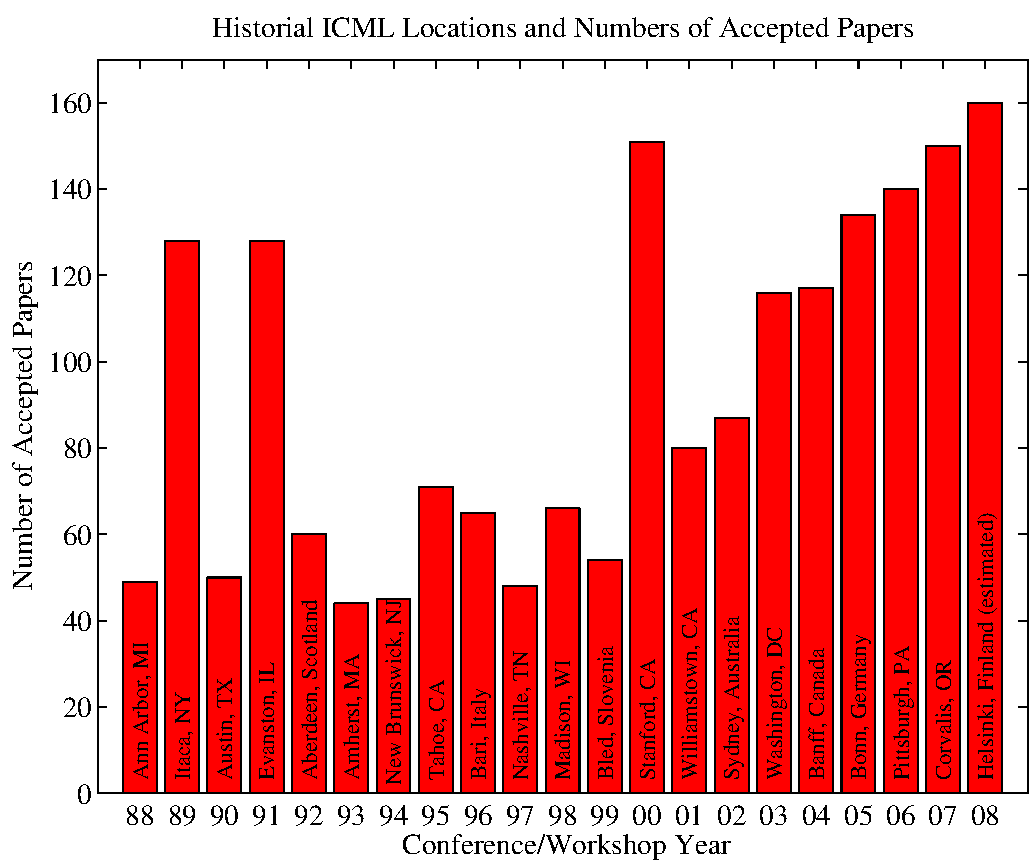
\includegraphics[width=\columnwidth]{icml_numpapers}}
% \caption{Historical locations and number of accepted papers for International
%   Machine Learning Conferences (ICML 1993 -- ICML 2008) and
%   International Workshops on Machine Learning (ML 1988 -- ML
%   1992). At the time this figure was produced, the number of
%   accepted papers for ICML 2008 was unknown and instead estimated.}
% \label{icml-historical}
% \end{center}
% \vskip -0.2in
% \end{figure}

% Quantitative
Interpretable embeddings.
Nearest neighbor analysis quantitatively show the defined partitions are preserved.

% Qualitative
Follow trajectories of sounds in 3-space.
Concatenative synthesis, qualitative analysis.



\section{Conclusions}

We have explored


Number figures sequentially, placing the figure number and caption
{\it after\/} the graphics, with at least 0.1~inches of space before
the caption and 0.1~inches after it, as in
Figure~\ref{icml-historical}.  The figure caption should be set in
9~point type and centered unless it runs two or more lines, in which
case it should be flush left.  You may float figures to the top or
bottom of a column, and you may set wide figures across both columns
(use the environment {\tt figure*} in \LaTeX), but always place
two-column figures at the top or bottom of the page.


% Acknowledgements should only appear in the accepted version.
% \section*{Acknowledgements}

% \textbf{Do not} include acknowledgements in the initial version of
% the paper submitted for blind review.

% If a paper is accepted, the final camera-ready version can (and
% probably should) include acknowledgements. In this case, please
% place such acknowledgements in an unnumbered section at the
% end of the paper. Typically, this will include thanks to reviewers
% who gave useful comments, to colleagues who contributed to the ideas,
% and to funding agencies and corporate sponsors that provided financial
% support.


% In the unusual situation where you want a paper to appear in the
% references without citing it in the main text, use \nocite
% \nocite{langley00}

\bibliography{example_paper}
\bibliographystyle{icml2016}

\end{document}


% This document was modified from the file originally made available by
% Pat Langley and Andrea Danyluk for ICML-2K. This version was
% created by Lise Getoor and Tobias Scheffer, it was slightly modified
% from the 2010 version by Thorsten Joachims & Johannes Fuernkranz,
% slightly modified from the 2009 version by Kiri Wagstaff and
% Sam Roweis's 2008 version, which is slightly modified from
% Prasad Tadepalli's 2007 version which is a lightly
% changed version of the previous year's version by Andrew Moore,
% which was in turn edited from those of Kristian Kersting and
% Codrina Lauth. Alex Smola contributed to the algorithmic style files.
